\chapter{Anexos}
\label{cap:anex}


\section{Museu da Pessoa — tratamento de fotografias}
\label{seq:anex-museu}


\subsection{Filtro de Texto}
\label{seq:anex-museu-filtro}


\subsection{Estrutura de dados}
\label{seq:anex-museu-est}


\subsection{Cabeçalho ficheiro C}
\label{seq:anex-museu-header}


\section{Processamento de Entidades Nomeadas (Enamex)}
\label{seq:anex-enamex}


\subsection{Filtro de Texto}
\label{seq:anex-enamex-filtro}


\subsection{Estrutura de dados}
\label{seq:anex-enamex-est}


\subsection{Cabeçalho ficheiro C}
\label{seq:anex-enamex-header}


\section{Processamento de ficheiros com Canções}
\label{seq:anex-music}


\subsection{Filtro de Texto}
\label{seq:anex-music-filtro}
\verbatiminput{2-5.flex}


\subsection{Estrutura de dados}
\label{seq:anex-music-est}
\begin{verbatim}
typedef struct sMusicLine {
    char* line;
    struct sMusicLine* next;
} MusicLine;

typedef struct sMusic {
    char* _Title;
    char* _From;
    char* _Author;
    char* _Lyrics;
    char* _Music;
    char* _Singer;

    MusicLine* poem;
    MusicLine* poemEnd;
    int error;
} Music;
\end{verbatim}


\subsection{Cabeçalho ficheiro C}
\label{seq:anex-music-header}
\verbatiminput{2-5.h}

\subsection{Testes}
\label{seq:anex-music-tests}
\subsubsection{Input teste 1}
\label{seq:anex-music-test-in01}
\verbatiminput{anexos/2-5-a-in}

\subsubsection{Output teste 1}
\label{seq:anex-music-test-out01}
\verbatiminput{anexos/2-5-a-out}

\subsubsection{Input teste 2}
\label{seq:anex-music-test-in02}
\verbatiminput{anexos/2-5-a-in}

\subsubsection{Output teste 2}
\label{seq:anex-music-test-out02}
\verbatiminput{anexos/2-5-b-out}

\subsubsection{Input teste 3}
\label{seq:anex-music-test-in03}
\verbatiminput{anexos/2-5-c-in}

\subsubsection{Output teste 3}
\label{seq:anex-music-test-out03}
\verbatiminput{anexos/2-5-c-out}

\begin{figure}
\centering
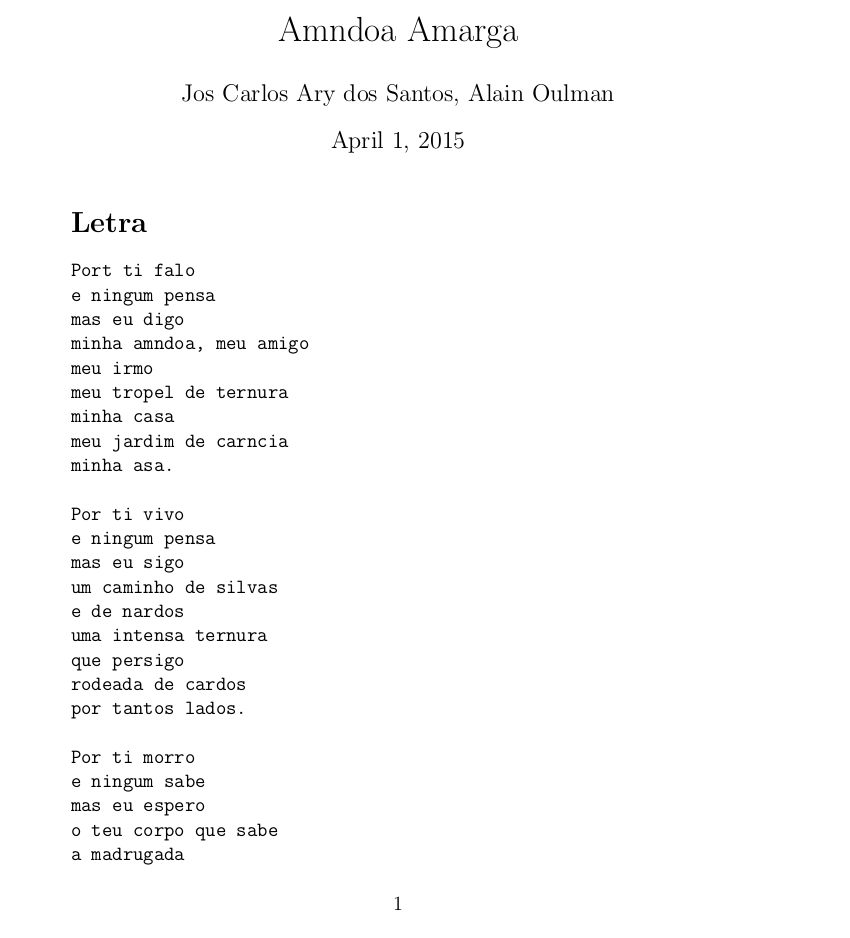
\includegraphics[width=15cm]{anexos/2-5-a-img1.png}
\caption{PDF gerado por o ficheiro latex (teste 1). Pagina 1 de 2}
\end{figure}

\begin{figure}
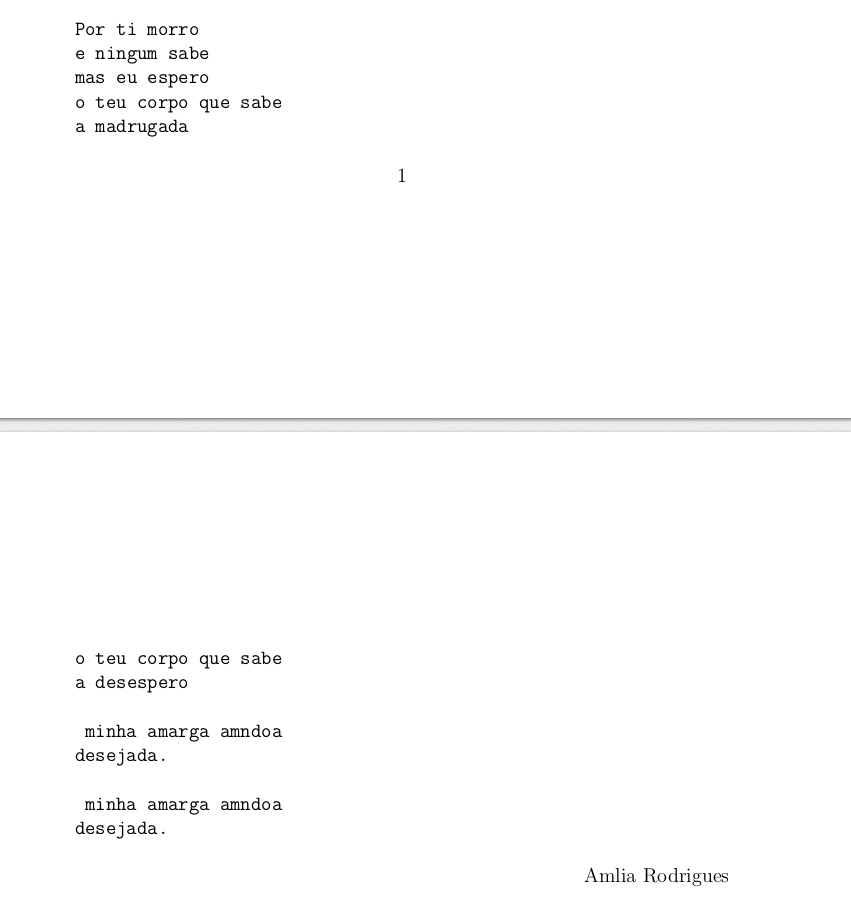
\includegraphics[width=15cm]{anexos/2-5-a-img2.png}
\caption{PDF gerado por o ficheiro latex (teste 1). Pagina 2 de 2}
\label{fig::anex-music-test-img}
\end{figure}

\begin{figure}
\centering
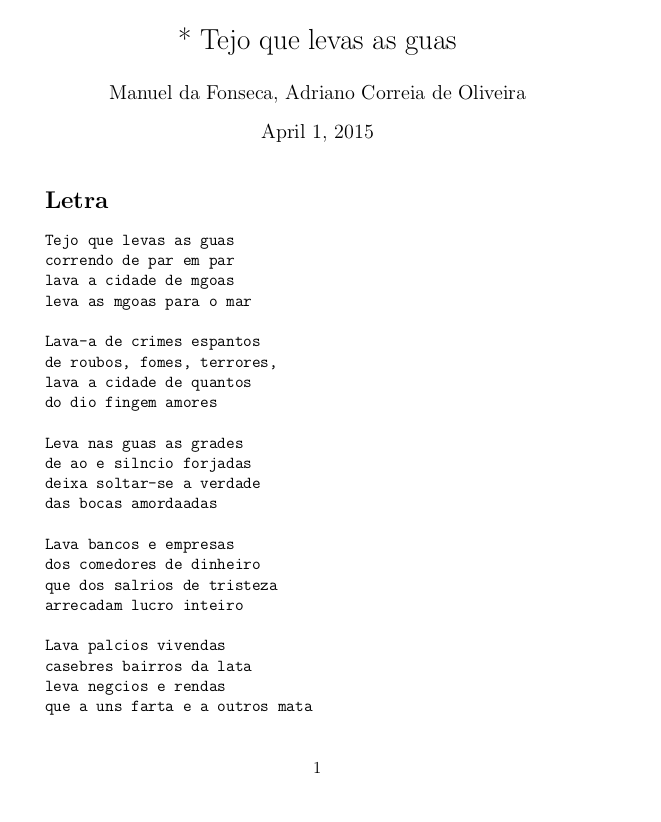
\includegraphics[width=15cm]{anexos/2-5-b-img.png}
\caption{PDF gerado por o ficheiro latex (teste 2). Pagina 1 de 2}
\label{fig::anex-music-test-img02}
\end{figure}

\begin{figure}
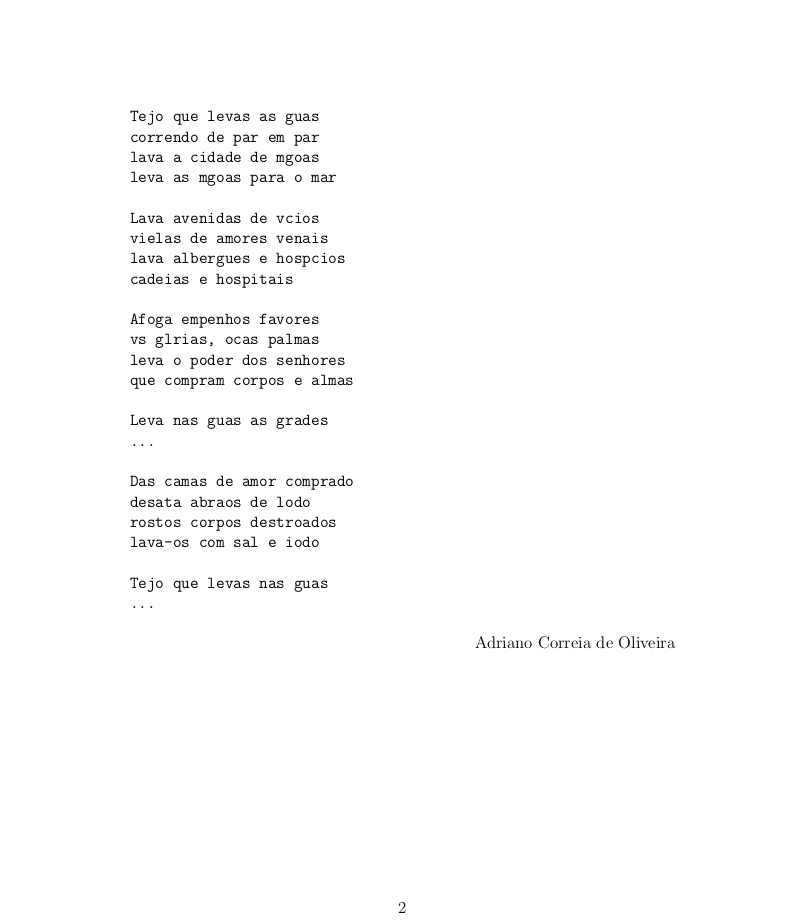
\includegraphics[width=15cm]{anexos/2-5-b-img2.png}
\caption{PDF gerado por o ficheiro latex (teste 2). Pagina 2 de 2}
\label{fig::anex-music-test-img}
\end{figure}


\begin{figure}
\centering
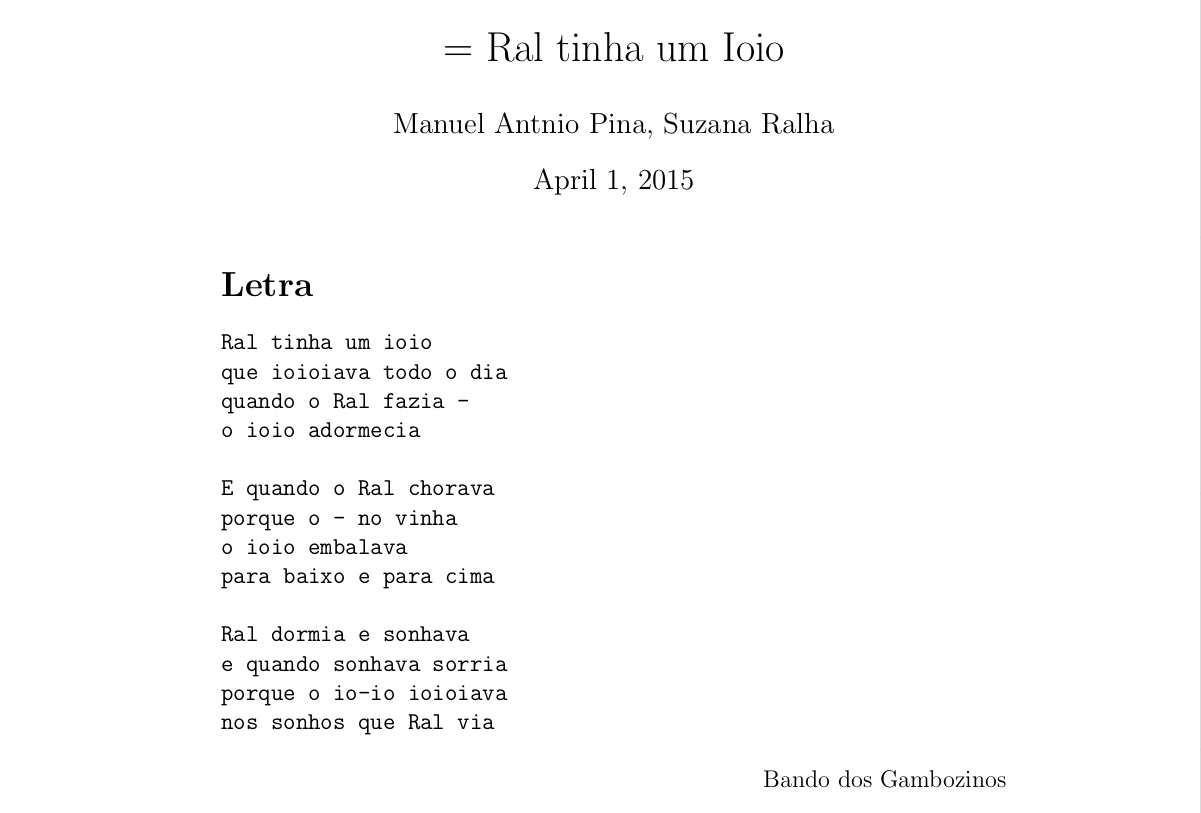
\includegraphics[width=15cm]{anexos/2-5-c-img.png}
\caption{PDF gerado por o ficheiro latex (teste 3)}
\label{fig::anex-music-test-img03}
\end{figure}